\chapter{Casebeskrivelse}
\label{chp:case}
Byggningen av det nye universitetssykehuset i Trondhein, St.Olavs Hospital ble påbegynt i 2003 og sto ferdig sommeren 2013. Byggingen ble fordelt på hovedsaklig to byggefaser, hvor avdelingene flyttet inn i sine nye omgivelser etter hver fase. Som en del av byggeprosjektet inngikk også det som da var Norges største, dyreste og mest kompliserte IKT-leveranse noensinne \citep{TU}. 

\noindent
Pasientsignalsystemet som brukes på sykehuset i dag var en del av denne levaransen, og ble utviklet spesielt for St.Olavs Hospital. Systemet skiller seg fra det som ble brukt tidligere, blandt annet i at pasientsignal kun ble varslet på paneler på vegg og i tak. Også knappen sykepleierne kunne bruke for å be kolleger om assistanse ble fjernet.

\noindent
I forkant av innflyttingen fikk de ansatte opplæring, blandt annet i hvordan det nye pasientsignalsystemet fungerte. Noen ansatte fikk mer omfattende opplæring, og ble superbrukere av systemet, med den hensikt å fungere som ambasadører for systemet, go hjelpe til med opplæring på avdelingene. Den første tiden etter at systemet var tatt i bruk var det også plassert $"$on site help desk$"$ på alle avdelinger for å svare på spørsmål og hjelpe til med bruk. I dag er det den enkelte avdeling som har ansvar opplæring av sine nyansatte. 

\noindent
Ved innflyttingen i nytt sykehus var det meningen at alle skulle bruke telefonen til å motta pasientsignaler. Det var derimot noen avdelinger, deriblandt avdeling A1, som viste sterk motstand og nektet å bruke telefonene til dette.
Høsten 2013 flyttet avdelingen inn i nye lokaler, og gikk i forbindelse med dette med på å bruke systemet slik det var tiltenkt i en prøveperiode på 14 dager. Etter denne prøveperioden gikk avdelingen likevel tilbake til å ikke motta pasientsignaler på telefon. 
I forbindelse med denne flyttingen fikk de også tilbake assistanseknappen de lenge hadde ønsket seg. Denne er plassert sammen med den grønne og røde knappen på panlet inne på pasientrommet, og brukes til å fortelle kolleger at man har behov for assistanse. Varslingen fra denne kanppen vises kun på veggpanelene og ikke på IMATISskjermen.

\noindent
Med det nye sykehuset ble utformingen av avdelingene endret. 
Avdelingene er delt i sengetun, hvor hvert sengetun normalt har seks til åtte pasientrom. Dette er en fysisk og funksjonell måte å organisere pasientrommene på, og for å sikre fleksibilitet og effektivitet ligger flere sengetun ved en sengepost etter hverandre i serie, som vist i figur \ref{fig:sengepost} \citep{Aslaksen, sykehuskart}. Sengetunene består av en arbeidsstasjon, nærlager, sengerom og bad. Mellom tunene ligger støtterom som blandt annet kjøkken og oppholdsrom for pasienter, medisinrom, skylle/avfallsrom og undersøkelsesrom. Et overordnet mål for en slik organisering er å redusere barrierer mellom pleier og pasient, bedre mulighet for overvåking av pasienter og redusert risiko for uønskede hendelser, noe som øker sikekrheten for pasientene \citep{Sintef-sengetun}.
Signalsystemet kan til en viss grad konfigureres på en slik måte at sykepleiere på et sengetun kan motta pasientsignaler fra andre sengetun \citep{Aslaksen}. 

\begin{figure}[H]
\centering
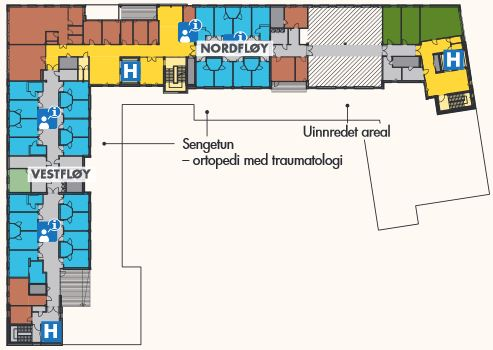
\includegraphics[scale=0.9]{bevegelse_6etg.jpg}
\caption{Sengepost inndelt i sengetun \citep{sykehuskart}. De blå områdene er sengetun/pasientrom, gule områder felles og brune omåder er støtterom.}
\label{fig:sengepost}
\end{figure}

\noindent
De åpne arbeidsstasjonene er utstyrt med PC'er, og fungerer som en desentralisering av vaktrommet. 

\begin{figure}[H]
\centering
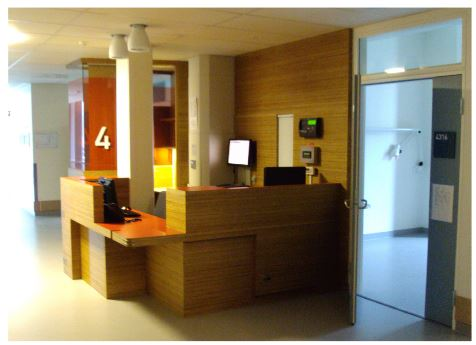
\includegraphics[scale=0.7]{Arbeidsstasjon.jpg}
\caption{Åpen arbeidsstasjon på sengetun \citep{sykehuskart}}
\label{fig:arbeidsstasjon}
\end{figure}

\noindent
På alle avdelingene forskerene har observert er delt inn i sengetun. Likevel skiller utformingen av avdeling A1 seg fra de to andre.
Avdelingene A2 og A3 er har tydelige sengetun, med pasientrommene plassert rundt arbeidsstasjonen, som i figur \ref{fig:sengepost}. På avdeling A1 er derimot pasientrommene plassert i en gang sammen med arbeidsstasjonene. 


\section{System}
En overodnet oversikt over hvordan vasling av pasientsignal fungerer er illustrert i figur \ref{fig:detteskjer}. En mer detaljert beskrivelse er veldlagt i tillegg \ref{chp:appendix_dagenssystem}.
Pasientene kan tilkalle sykepleier blandt annet ved å trekke i snoren på anropspanelet, som er montert på veggen ved sengen. Signalet varsles da via vaktromsapparatet som henger synlig på sengetunet, og via rompaneler på de pasientrom hvor sykepleiere er tilstedemarkert (denne markeringen gjøres ved at sykepleier trykker på den grønne knappen på rompanelet). 

\noindent
Sykepleierne skal registrere seg i bemanningsplanen i begynnelsen av skiftet. Denne gir pleierne muligheten til å selv påvirke hvordan pasientsignalene skal distribueres. Pleiere har mulighet til å registrere seg som primær- og/eller disponibel på pasientrom og som disponibel på hele eget eller andre tun. Et utløst pasientsignal vil først varsles på telefon til den pleieren som er registrert som psrimær på det aktuelle rommet. Dersom signalet ikke blir godtatt vil det gå videre til disponible pleiere. Signalet vil fortsette i denne løkken til det blir besvart.
Ved et innkommende pasientsignal kan sykepleieren velge å godta eller avvise signalet på telefonen. Dersom pleieren velger å avvise sigalet, eller ingen valg gjøres innen 15 sekunder sendes signalet videre til neste pleier på bemanningsplanen, som settes opp og konfigureres på PC'en på sengetunet. Dersom pleierene velger å godta signalet blir dette lagt i arbeidslisten på telefonen, og pleieren har 120 sekunder på seg til å tilstedemarkere seg på det aktuelle pasientrommet \citep{BrukermanualforPasientsignalogPasientsignalapplikasjon}.

\begin{figure}[H]
\centering
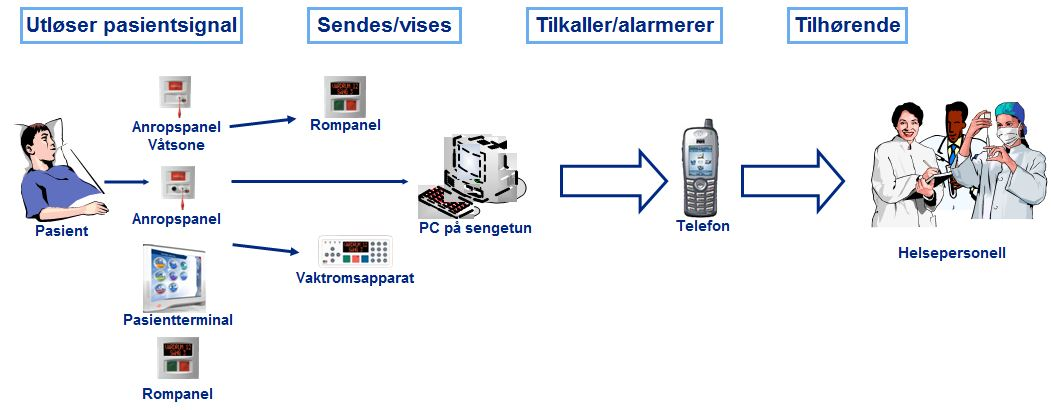
\includegraphics[scale=0.5]{alarmprosess.jpg}
\caption{Dette skjer ved utløst pasientsignal.}
\label{fig:detteskjer}
\end{figure}

\noindent
Der de samme signalene varsles på veggpanelene og på telefon, fører en forsinkelse i det trådløse systemet til at signalet varsles tidligere på veggpanelene. Dette har forskerene selv observert, og blitt bekreftet gjennom intervjuene. Det foreligger desverre ingen tall på hvor stor forsinkelsen er. 

\noindent
Vaslingssystemt består av et fast og et trådløst system, hvor det faste består av veggpanelene, mens det trådløse består av de trådløse IP-telefonene og IMATIS-skjermene. Det faste systemet er konfigurert i fysiske, kablede sløyfer som kobler sammen sengetun og gjør det mulig å motta vaslinger fra andre tun på veggpanelene. I tilfeller hvor man ønsker å motta signaler fra tun som er koblet til andre sløyfer enn en selv må pleierene motta disse på sin telefon, da dette kan konfigureres gjennom bemanningsplanen.